\documentclass[a4paper]{jsarticle}
\usepackage{iapaper}
\usepackage[dvipdfmx]{graphicx}


\begin{document}
% 修士論文の場合は \degreethesis を使わず,下記を使う.
% なお博士の場合は \doctorthesisにすること
 \masterthesis
% 卒業論文の場合は下記を使う
% \degreethesis


\title{論 文 題 目}
\date{平成28年度}
\advisor{渡邉英徳} % 指導教員名を入れる
\IDnumber{15893507}
\Mauthor{木村汐里}% 自分の名前を入れる.修士の場合は \Mauthor{氏名} に変更する.
\submissiondate{平成29年1月25日}
\maketitle


\pagenumbering{roman} % 要旨はRoman書体で表示
\setcounter{page}{1} % 1から振り直す
\jasummary{論文タイトル}{副題(必要であれば記入)}
ここには日本語文章のみで論文要旨を記述してください。
\summary{Title}{Subtitle}
The author shall write a thesis in English text. 150 words.

\makemokuji


\newpage

\pagenumbering{arabic}  % 論文本体はArabicで表示
\setcounter{page}{1} % ページ番号を1から振り直す
\section{序論}
本研究の概要, 背景と研究目的について述べ,本論文の構成について説明する.
\subsection{本研究の概要}
本研究では,集落組織が弱体化した過疎地域における「対話と交流の“場”」を形成する手法について検討する。そのために,新潟県魚沼市の過疎地域である横根地区に実際に滞在し,住民とともに“場”の形成を実践する.
まず,先行研究や先行事例を整理し、限界集落における地域活性化の活動における「対話と交流の“場”」の位置付けを明らかにする. さらにワークショップ手法の先行事例について検討し,”場”における話題を促進するコンテンツと,世代・性別ごとの参加プロセスに注視することの重要性を導き出す.
この結論に基づき,過疎地域における「対話と交流の“場”」のプログラムデザインを設計する.実際の集落においてこのプログラムを用いて“場”の形成を実践を通して比較検証した結果,地域の多様な世代が参加し,活発な意見が交換される場が形成された.さらに,活動の内容をSNSで地域外に発信し,広く共有することによって,地域内外が相互作用を生む場も形成された.
このことから,創出したプログラムデザイン手法は妥当であり、過疎地域における対話と交流の“場”が形成を促されたといえる.これは,専門家でなくとも利用可能であり今後,国内に増えていくと予想される限界集落における諸問題を解決するための,一つのモデルとなりうる.
\subsection{背景と課題}
\subsubsection{地域活性化における内発的発展}
近年,地域活性化は国土政策における重要な課題となっており,なかでも、条件不利地域の維持に関する調査は,論点や調査方法こそ異なるが,各省庁によって(国土交通省\cite{1},)実施されている.このような現状に対して,まち・ひと・しごと創生本部や内閣府地方創生推進事務局の設置などを皮切りに、国土交通省重点政策\cite{2}の策定を始め,地域おこし協力隊の派遣など国や自治体による政策・支援活動も数多く実施されている.しかし,トップダウンの財源と人的リソースは限られていることもあり,依然として担い手の確保の状況は厳しく,地域からの内発的な発展が強く求められている.
\subsubsection{過疎地域における「地域コミュニティ問題」の現状}
過疎化とは、簡単にいうと地域の人口 (戸数)が急減し、そのことで産業の衰 退や生活環境の悪化がもたらされ、住民意識が低下し、最後には地域から人がいなくなる(集落が消滅する)ことと捉えられる。\cite{3}これは、農林水産業等の第一次産業から第二・三次産業へ の移行とそれに伴う農村部から都市部への人口移動という中で、すでに1960年代の高度経済成長期から「問題」として捉えられてきた.\cite{4}さらに山下は、「過疎問題」という 問題提起そのものが政治・行政によってなされ、財政的支援による中央との格差是正として解決が求められていくことで、結果として、過疎地域自身が問題を内発的に解決せずに、 地域はつねに政策の客体=受け手として振る舞うよう習慣化されてきたことを指摘している.\cite{5}
 さらに過疎地域の地域コミュニティでは,集落組織の弱体化が進んでおり、機会の減少や閉鎖的な空間であること、変化がおこりにくいなどの過疎集落の特徴がある。これらの特徴から地域の現在と未来に対して悲観的になり、集落機能や集落そのものの維持に対する関心を失い、それが結果として実際に集落機能や地域ネットワーク、集落そのものの喪失を早めるという、「負のスパイラル」ともいうべき現象が起きていると言われている。\cite{6}ゆえに、集落の人々が主体的に取り組む気持ちの涵養が重要視され、集落に居住していない人々、その地の出身者や近くの集落、また中心都市の人々を、集落に積極的に関わらせていく必要があると山下は論じている。\cite{7}


\section{本研究の目的}
筆者はこれまでに述べた背景を踏まえ、過疎地域の内発的な発展を推進するために必要不可欠である地域再生にむけた地域住民のモチベーションを高めるため、「対話と交流の場」を過疎集落において形成する手法について考察する。そこで以下のように目的と達成要件を定義した.

\section{論文の構成}
論文は本論を含め以下の1--8の項目を含むこと。
\begin{enumerate}
\item 表紙 … 論文全体の内容を表す表題、指導教員名、提出年月日、学修番号、氏名等を記載すること。
\item 要約 … 論文全体の要約を和文2000 字程度、英文150語程度で記述すること。研究の背景、目的、実施内容、その手法と結果、結論を簡単明瞭に網羅すること。
\item 目次 … 論文の章・節の番号とその表題およびページを記入すること。
\item 序論 … 論文の第1章では序論として、その分野における本研究の位置付け、歴史的背景、本研究の目的を述べること。本研究が従来の研究とどういう関係にあり、どのような点を明らかにすることを目的とするか、本研究がどういう点で新しいかを明確に述べる必要がある。
\item 本論
\item 結論 … 論文の最後の章に結論を設けること。研究目標に対してこの研究がどこまで到達できたかを検討し簡単に記述すること。また、本研究で成し得なかった事項、今後の課題等も述べるとよい。
\item 謝辞… 研究を遂行する際、援助・協力等があった場合、必要に応じて謝辞を記すこと。
\item 参考文献 … 研究内容に直接関係のある文献、引用した文献等は必ずその出処を明らかにすること。

各項目は節で構成される。具体的には section を利用する。副節は subsection を利用する。
\end{enumerate}

\section{論文のフォーマット}
\subsection{レイアウト:Microsoft Word}
用紙のサイズはA4.印刷は片面印刷とし、余白は上35mm、他下左右30mmとし、ヘッダーの用紙の端からの距離は15mm、ヘッダーのそれは17.5mmとします。
Microsoft Wordの標準設定であり、Microsoft Wordの使用者は特に設定する必要はないです.用紙の確認は、「ファイル」メニューより「ページ設定」、余白と用紙サイズが以下のようになっているかを確認します。本文の日本語フォント種類はMS明朝、英語フォントはTimes New Romanとします.フォントの大きさは10.5ポイント.本文中で使用する英語や数字は基本的に半角文字とします(表記が論文内で統一されていればどちらでもよい).また、句読点「 、 . 、 。 」も論文内で統一します。
論文のレイアウトは、A4文字の大きさは12ptとし、1行当たりの字数を40字、行数を30行とする。修士論文の場合50ページ程度を標準とする。用紙の下中央に連続したページ番号を付けること。

\subsection{レイアウト: \TeX}
原則は、上記で示したMicrosoft Wordの形式の通りとなります。ただし字数に関しては \TeX が最適な字間を決定するため、あくまで40字は目安となります。

\subsection{図表の入れ方}
図は figure 、表は table にて挿入する。図\ref{fig:tmu_hino}は日野キャンパス外観を示す。本稿で利用できる画像形式は jpg, png を中心に利用されたい。ただしEPS, TIFF も利用できる。どちらの場合も解像度を考慮してデータを作成すること。
\begin{figure}[tb]
  \begin{center}
    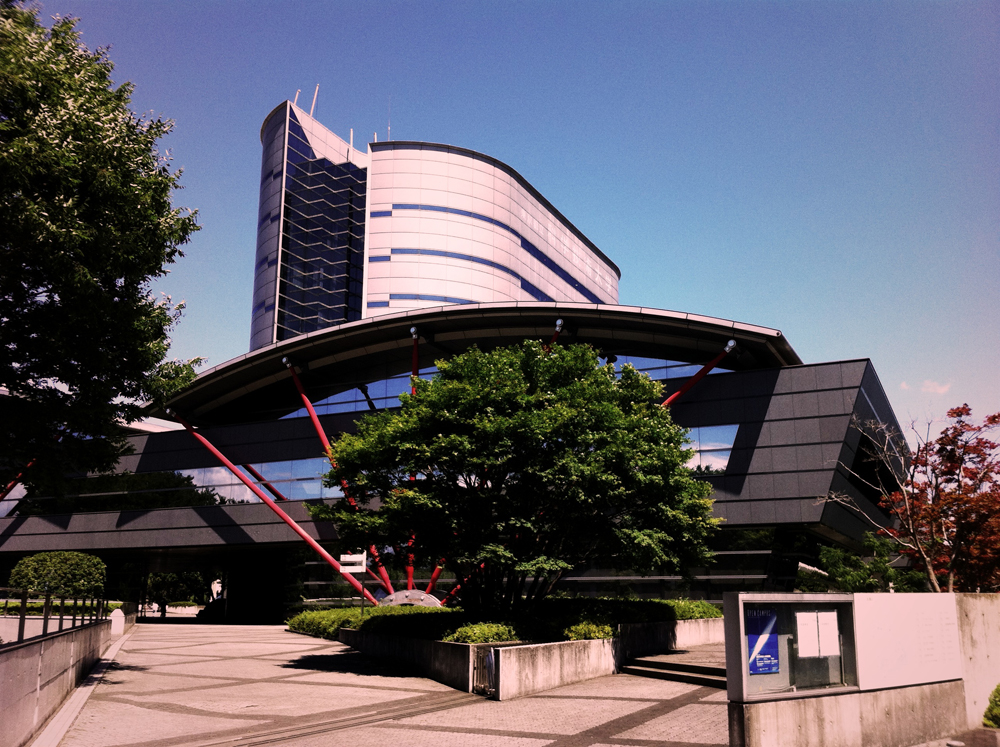
\includegraphics[width=0.95\hsize]{./images/sample.jpg}
    \caption{首都大学東京日野キャンパス}
    \label{fig:tmu_hino}
  \end{center}
\end{figure}

図を複数枚横に並べて表示したい場合は、minipage を利用する。と図\ref{fig:tmu_hino_yokonarabi}の様に表示できる。

\begin{figure}[tb]
  \begin{center}
    \begin{tabular}{ccc}

    \begin{minipage}{0.3\hsize}
	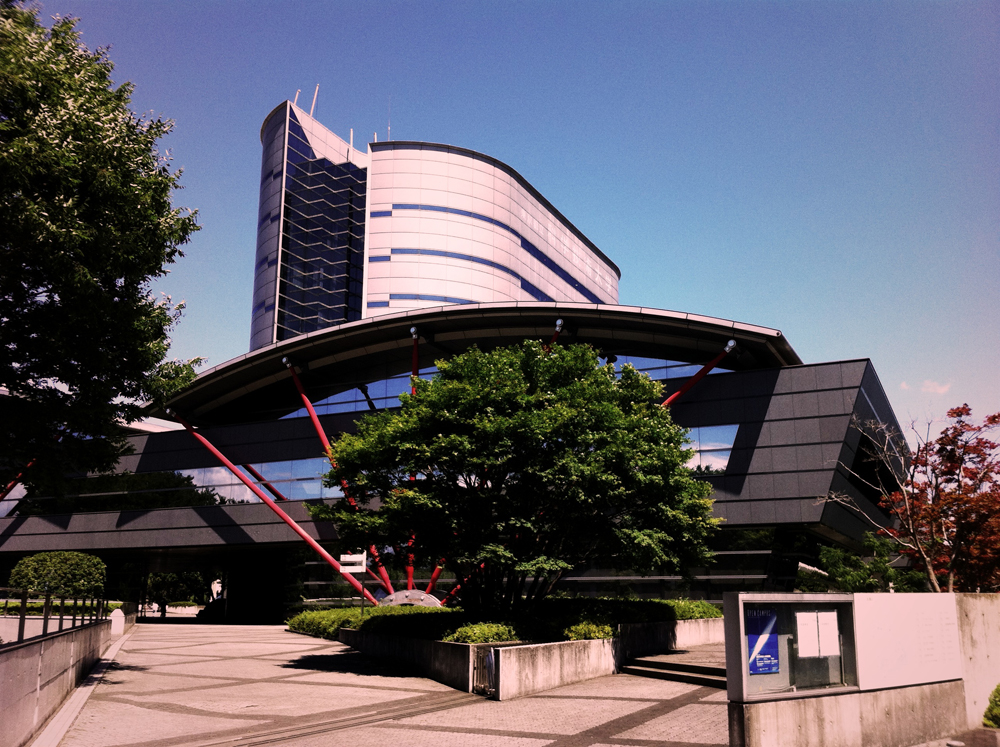
\includegraphics[width=\hsize]{./images/sample.jpg}
    \end{minipage}
    &
    \begin{minipage}{0.3\hsize}
      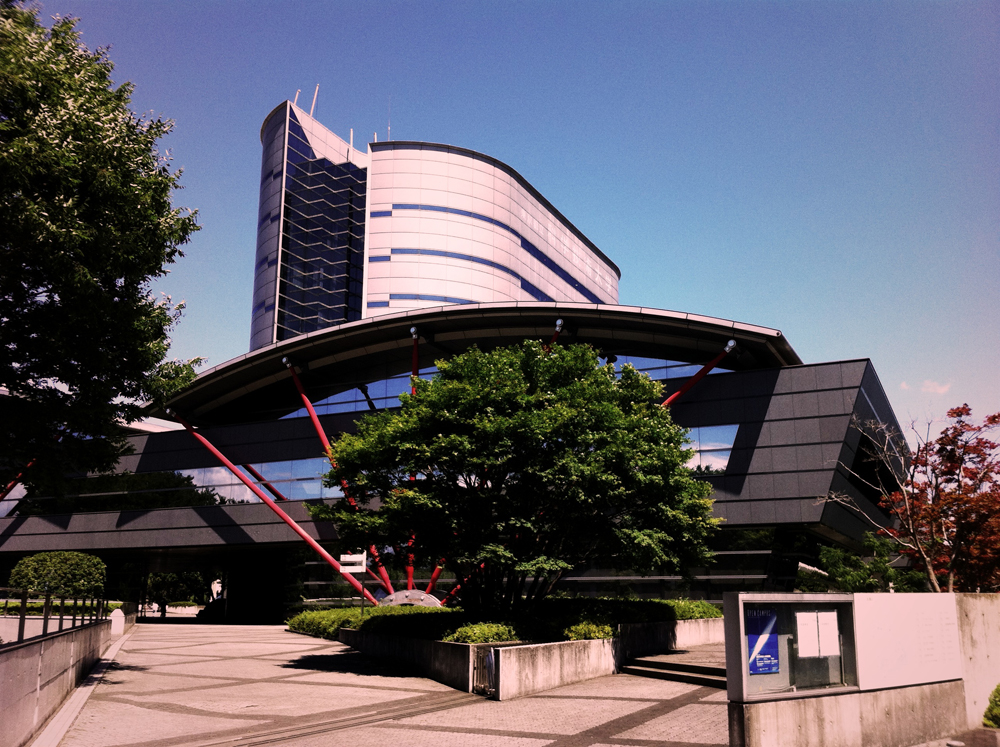
\includegraphics[width=\hsize]{./images/sample.jpg}
    \end{minipage}
    &
    \begin{minipage}{0.3\hsize}
      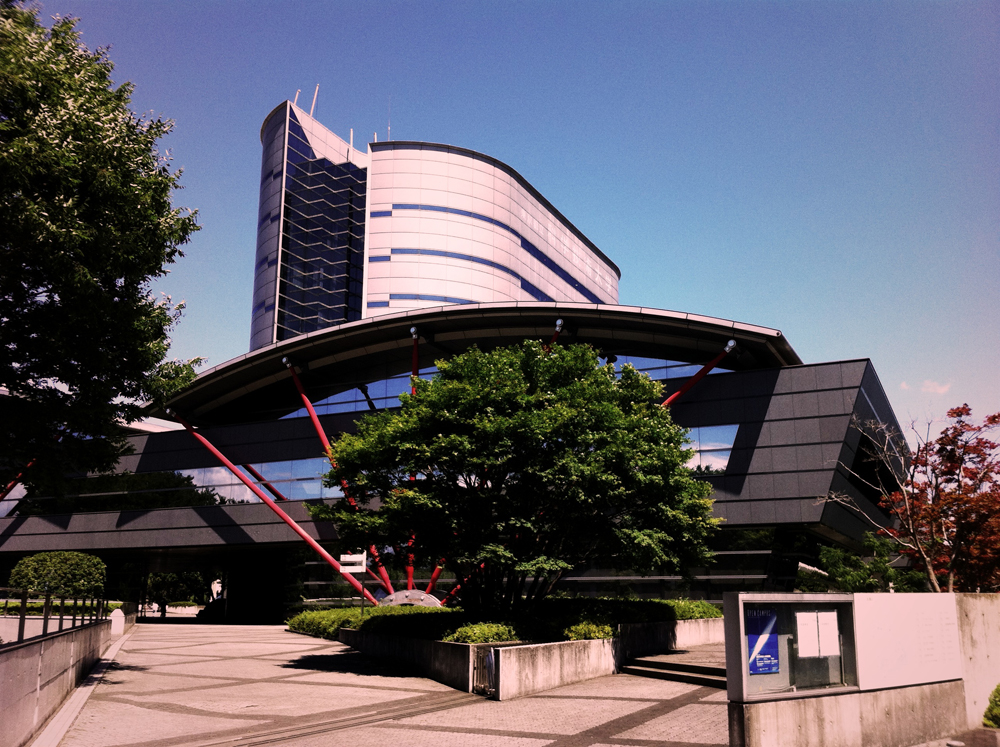
\includegraphics[width=\hsize]{./images/sample.jpg}
    \end{minipage}

  \end{tabular}
    \caption{日野キャンパス横並び}
    \label{fig:tmu_hino_yokonarabi}
  \end{center}
\end{figure}


論文の中に図や表を貼り付ける際には図表1、2のように表組みを利用して縦横に複数並べるか、あるいは、図表3のように図表の左右に本文を流し込まないようにします。そのためには、図(表)を右クリックして現れる、書式設定内の「レイアウト」タグを「行内」に設定します(図3を参照)。図や表の配置は、その大きさと文章とページの空き具合で次のページに自動的に移動されます。また、文章領域内におさまるように絵の大きさを調整します。

\subsection{参考文献の書き方}
参考文献は、ジャーナルの場合、著者名・タイトル・雑誌名・巻号・ページ・発行年、著書の場合は、著者名・書名・発行所・発行年、以上の順に書くこと。著者が複数の場合も略さず全著者名を記入すること。これに関しても分野によっては、記述形式・記述順番が異なるので、指導教員にあらかじめ確認してください。\TeX では文献を thebibliography 以下に列挙し、リスト名を作っておくことで、適時\cite{sample} などとcitationができる。なお参考文献の作成の仕方は幾つかあり、下記の記述方法はユーザが手動で入力する方法である。

\begin{thebibliography}{999}
  \bibitem{1}
  著者名1,著者名2
  論文タイトル名、
  発表シンポジウム・会議名、
  発表学会名、
  記事番号やページ、
  発表年
  \bibitem{2}
  著者名1,著者名2
  論文タイトル名、
  発表シンポジウム・会議名、
  発表学会名、
  記事番号やページ、
  発表年
  \bibitem{3}
  著者名1,著者名2
  論文タイトル名、
  発表シンポジウム・会議名、
  発表学会名、
  記事番号やページ、
  発表年
  \bibitem{4}
  著者名1,著者名2
  論文タイトル名、
  発表シンポジウム・会議名、
  発表学会名、
  記事番号やページ、
  発表年
  \bibitem{5}
  著者名1,著者名2
  論文タイトル名、
  発表シンポジウム・会議名、
  発表学会名、
  記事番号やページ、
  発表年

\end{thebibliography}

\section*{論文の提出期限}
大学院は大学院教務委員に確認し、学部生は指導教員に確認してください。
\end{document}
